% !TeX root = ../main.tex
\chapter{Broadband photon pair generation}

Back to the classical nonlinear optics theory, the solution to nonlinear coupling equations requires the initial power at ether signal or idler mode, which is called seed in the laser terminology. However, in quantum optics theory, all the modes in cavity behave intrinsic vacuum fluctuation at the quantity of half $ \hbar \omega $. Thus, even without light fed, the quantum fluctuation leads to emission at the single photon levels. 

Furthermore, intracavity pump power then behaves the amplifier, intensify the corresponding signal or idler mode photon flux. Once the single photon flux exceeds cavity threshold, the extracavity single photon can be detected. To note, these kind of excitation is indistinguishable because the signal and idler photons are emitted simultaneously as a result of quantum mechanics, rather than signal photon stimulates idler photon and vice versa. In the context of quantum states, the state created intracavity is at the superposition of signal state and idler state. The wave packet is different from the normal single photon one. Further theoretical research \cite{Scully1997} explained the squeezed nature of four wave mixing photon pairs, which is one of the exclusive properties of frequency entangled photon pairs.

In general, the spontaneous four wave mixing in nonlinear cavities defined in our context refers to the cavity modes are excited collectively and pair-by-pair under the phase matching condition. Thus, under the weak coherent approximation, the photon pair only include one photon in each mode but correlated with each other. Thus, the conventional coincidence counting technology can be used to verify such correlation. In the term of generation band, it agrees with the classical phase matching condition at pump power limit.

%Furthermore, 
%To clarify with the physics compared with the relevant research, such as Kerr frequency comb and soliton generation, where ultra-high power is used to built intracavity pump mode, the spontaneous four wave mixing differs 
%\cite{Chembo2016a}

\section{Methods}

Using the dispersion extraction method in previous chapter, zero dispersion wavelength can be located easily among the measured band. In our experiments, optical telecom band, especially C band is focused on, because enormous fiber optical components, like in-line filters are available in this range.

Illustrated in \autoref{fig:bibpf}, the setup of mode-resolvable singular photon pair generation first adopts the tunable laser as pump source, whose display tunability is 0.1 pm and able to be tuned via external voltage input. The laser output is connected to ring resonators using the fiber launching system and the output power is measured with the power meter. 

A simple transmission scanning is then perform to select the built-in polarization.
For the high \textit{Q}-factor devices, the transmission of TE and TM modes are separated in a distance of tens of pm. Thus, as either of the resonance vanished by rotating the polarization controller, the fiber launches the particular polarization mode of bus waveguide. For low \textit{Q}-factor cavities, since the TE and TM are degenerate in the spectrum, the method of polarization alignment is as same as the one using the InGaAs infrared camera.

Beyond the polarization selection, the pump wavelength should also be aligned to the resonance of ring resonators. The on-resonance or off-resonance can be determined as the output displays largest distinction ratio. In our experiment, the pump peak around 1550 nm, usually perform at least 10 dB extinction ratio between on-resonance and off-resonance.

Next, the output light are splitted 50\si{\percent} by 50\si{\percent} into signal and idler channels, indicating half of generated photons are lost. The two channels are sequentially filtered through two sets of band pass filters. The 3dB bandwidth in the first set is 1540$\pm$4 nm and 1560$\pm$4 nm, respectively. The second set of band pass filters are 0.01nm-tunable and 3dB bandwith is 0.12nm. Since mode spacing, FSR in our device is much more larger, the tunable band pass filter is adequate to pass only single mode.

Finally, each channel are detected by superconducting single photon detectors (SNSPD) which are specific for infrared range. The time resolution is 100 ps. Since the SNSPD is polarization-sensitive, another two polarization controllers (not shown) are used to achieve maximal single photon counting during each measurement. At last, the time controller (ID Quantique, ID900) collects and records the counting time tag in the 100 ps resolution. The coincidence counting is triggered directly or calculated by setting the coincidence window. 

\begin{figure}
	\centering
	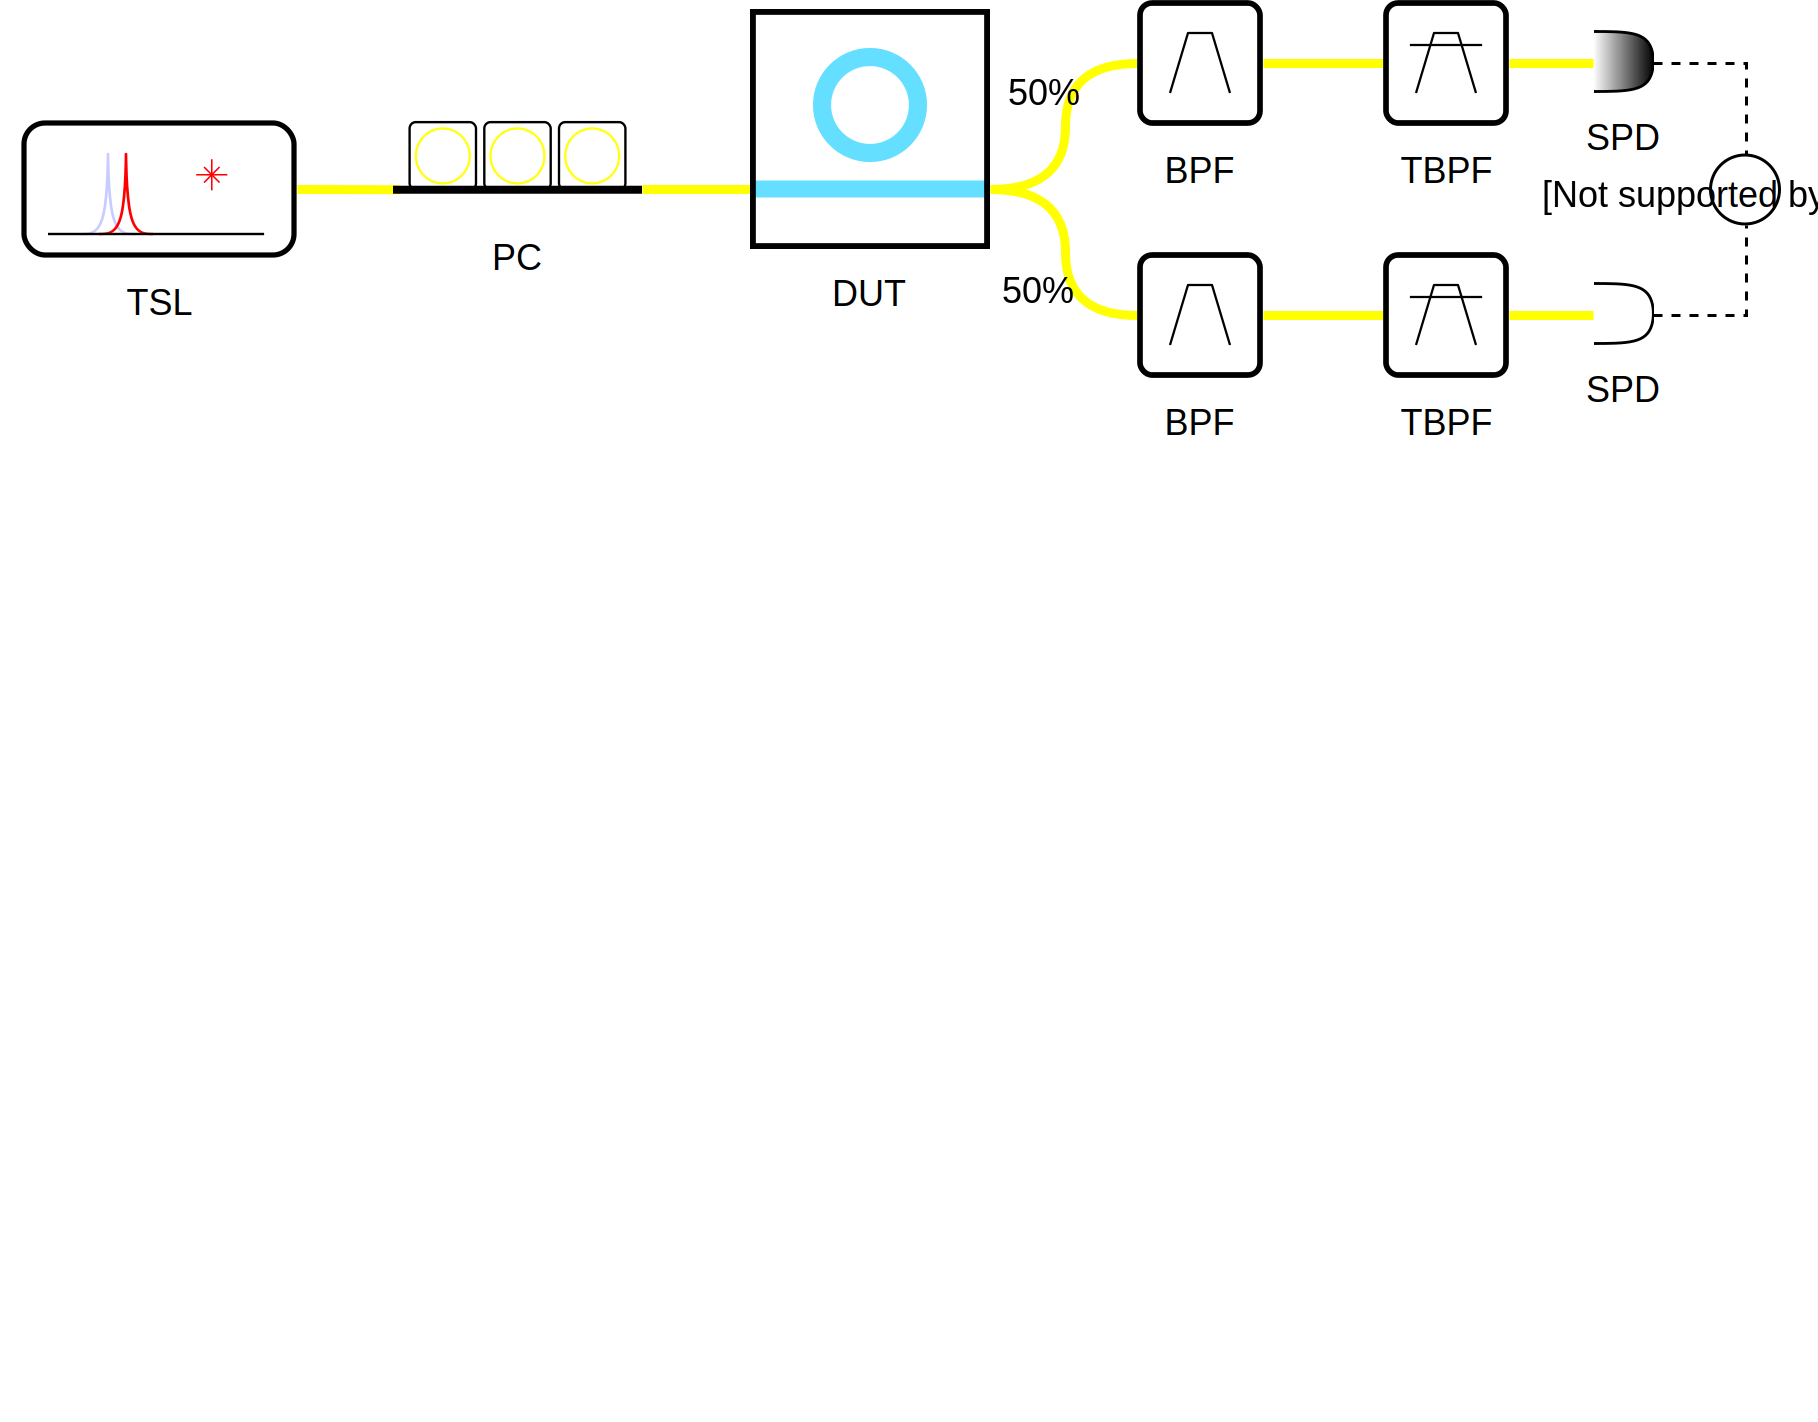
\includegraphics[width=1\linewidth]{imgs/biBPF.pdf}
%	\includesvg[width=.9\textwidth]{setup/biBPF}
	\mycaption{Mode-resolvable singular photon pair generation}{}
	\label{fig:bibpf}
\end{figure}

\bigskip
\textbf{Coincidence counting}

In quantum optics, coincidence counting is usually used to examine the non-locality of singular wave-particle. In our case, the photons which are splitted into two channels A and B yields the count per second $N_\mathrm{A}$ and $ N_\mathrm{B} $. Define the coincidence windows $t$, 1 ns commonly, and coincidence count (CC) is two photon trigger events within this small time window, equivalent to the photon pair generation rate effectively. The accidental counting (ACC) is defined as $ N_\mathrm{A} N_\mathrm{B} t $, similar to the background noise of counting system. Thus accidental-coincidence ratio (CAR) is defined as (CC-ACC)/ACC to reduce the noise effects.

It is worth to mention that in our research, the main topic is photon pair generation rather than photn state manipulation, in result numerous band-pass filters are exploited to realize mode-resolvable single photon counting. It does not contradict with distinguishability nature of frequency correlated photon pairs.


\section{Low power photon pair generation}

\subsection{Single mode photon flux}

With the pump power set as 100 \si{\micro\watt} and central wavelength at 1550.64 nm, the result of photon flux of both signal and idler bands versus relative mode index is presented in \autoref{fig:flux1}. The device deployed has FSR of 150 GHz and shows anomalous dispersion around 1550 nm. According to the 3dB bandwidth of band pass filters, the accessible relative mode index corresponds 7-14. To achieve higher photon counting, the central wavelength of TBPFs is tuned carefully in the step of 0.01 nm.

In the result, there is trend that both signal and idler photon fluxes decreases as the mode index increases. It can be explained that phase mismatch of farther modes is greater than closer ones. The difference between signal and idler bands origins from the asymmetry of phase matching condition and filter spectral shape. As the input power is set as 100 \si{\micro\watt}, the estimated photon generation rate is around \num{d3} per mode per \si{\micro\watt}.

\begin{figure}
	\centering
	\includesvg[width=5in]{mode_depen/flux_1}
	\mycaption{Photon flux at 100 \si{\micro\watt} of Ligentec group 2 device 1}{The pump power set as 100 \si{\micro\watt} and central pump wavelength is at 1550.64 nm. Selected modes is from 1536 nm to 1544 nm for idler band and 1556 nm to 1564 nm for signal band.}
	\label{fig:flux1}
\end{figure}


\subsection{Coincidence counts of singular mode pair}

In coincidence counts are measured in a 1ns coincidence window and in each mode, the time delay is set from -200 to 200 ps. The \autoref{fig:mode_cf} shows the result of coincidence counts and CAR. In the mode pair 9, single photo pair generation rate is 1500 per second, equals to \num{1.5d4} per mW, which is the highest rate observed at this input power level among all the samples.

As the mode number increases, coincidence counts varies roughly but in the CAR graph, such a trend is not obvious. This is due to the band pass filters used in our setup is not flat-top on the transmission spectrum. In conclusion, even several frequency-dependent optical components used in our setup, by calculating the coincidence-accidental ratio, the photon pair generation behavior can be analyzed precisely.

\begin{figure}
	\centering
	\includesvg[width=6in]{mode_depen/mode_cf}
	\mycaption{Photon flux at 100 \si{\micro\watt} of Ligentec group 2 device 1}{}
	\label{fig:mode_cf}
\end{figure}

\section{Pump power dependence}

Since the spontaneous four wave mixing originates from Kerr nonlinearity, in classical nonlinear optics, converted power is linearly dependent on pump power. To confirm this relation in quantum scale, it is necessary to study both power dependence of photon flux and coincidence counts.

To amplify the pump power, a erbium-doped fiber amplifier (EDFA) is cascaded after the tunable laser. By increasing the output power, the power intracavity can exceed 500 mW. 
The mode passed through is fixed at $ \mu=9 $ ,corresponding to $\lambda_\mathrm{i}$ = 1540.28 nm and $\lambda_\mathrm{s}$ = 1558.79 nm. During each peak resonance alignment, the extinction ratio is around 10 dB. 
The result of photo flux is given in \autoref{fig:pwflux}. It is apparent that there is a continual growth of photon flux in both signal and idler modes. 

\begin{figure}
	\centering
	\includesvg[width=3in]{pw_depen/pw_flux}
	\mycaption{}{}
	\label{fig:pwflux}
\end{figure}

\begin{figure}
	\centering
	\includesvg[width=6in]{pw_depen/pw_cc_acc}
	\mycaption{}{}
	\label{fig:pwcar}
\end{figure}

Furthermore, the coincidence counting result is shown in \autoref{fig:pwcar}(a) where both maximal coincidence counts and background accidental coincidence counts increase with the pump power. While from CAR provided in \autoref{fig:pwcar}(b), higher input power leads to a significant decline. This can explained by the background noise arising from the Raman effect in optical fibers \cite{Engin2012}
. As the nonlinearity of optical fiber is much weaker than silicon nitride device, in the high input power regime, it becomes obvious and contributes to the single photo count while decreasing the coincidence count rate.

\section{Joint spectrum intensity}

Since the spontaneous four wave mixing occurs simultaneously at each mode pair, the state generated in a broadband is equivalent to the intensity superposition all over the signal and idler bands. To clarify the quantum state characteristics in this view, usually the joint spectrum filed or intensity is measured to evaluate the frequency correlation \cites{Helt2010,Vernon2015b}. For example, compared with the $ N $ mode correlation measurement mentioned above, the joint spectrum intensity requires the coincidence measurement over the whole two-party $ N^2 $ hibert space.

\subsection{Setups}

Much of recent research concerning soliton generation discussed the thermal stability in the nonlinear ring resonators \cites{Guo2017a,Herr2012}. 

To solve this problem, illustrated in \autoref{fig:pid}, an auxiliary photon detector is added to monitor off-resonance. Using digital proportional–integral–derivative (PID) controller, which is realize by a LabVIEW program, the wavelength of tunable laser is tuned dynamically by the external voltage input. In this way, the extinction ratio of our system can keep at a low level as soon as possible. In addition, to increase the available mode number, the first set of band pass filter in \autoref{fig:bibpf} is replaced by a notch filter. 

\begin{figure}
	\centering
	\includegraphics[width=1\linewidth]{imgs/pid.pdf}
	%	\includesvg[width=.9\textwidth]{setup/biBPF}
	\caption{}
	\label{fig:pid}
\end{figure}

\autoref{fig:jsi} presents the final results of intermodal coincidence counts, accidental coincidence counts and their ratio, CAR. The operation 

\begin{figure}
	\centering
	\includesvg[width=5in]{jsi/flux_2}
	\mycaption{Photon flux at 100 \si{\micro\watt} of Ligentec group 2 device 1}{}
	\label{fig:flux2}
\end{figure}

\begin{figure}
	\centering
	\includesvg[width=6in]{jsi/jsi_map}
	\mycaption{}{}
	\label{fig:jsi}
\end{figure}



